This chapter explains some of the foundations necessary for understanding the core idea. These basics facilitate the reading of this work and the results from this chapter are required for further calculations. 

\section{Colour factor calculation}
\label{col}
The calculation of the Casimir operators of the respective diagrams must be dealt with in detail here, which occur later with the evaluation of the matrix elements. The generalization of the Pauli matrices are the so-called Gell-Mann matrices $\lambda ^a$ which are given by \cite{Schwartz:2013pla, Platzer:2018pmd}
\begin{equation}
\begin{split}
T^a =  \frac{\lambda ^2}{2}
\end{split}
\end{equation}

\begin{equation}
\begin{split}
\lambda ^1 =\begin{pmatrix} 0& 1 &\\ 1& 0 &\\ & & 0 \end{pmatrix},\:\:\: \lambda ^2 =\begin{pmatrix} 0& -i &\\ i& 0 &\\ & & 0 \end{pmatrix}, 
\:\:\: \lambda ^3 =\begin{pmatrix} 1&  &\\ & -1 &\\ & & 0 \end{pmatrix}, \:\:\: \lambda ^4 =\begin{pmatrix} &  &1\\ & 0&\\1 & &  \end{pmatrix}\\\
\lambda ^5 =\begin{pmatrix} &  &-i\\ & 0 &\\ i& &  \end{pmatrix},\:\:\: \lambda ^6 =\begin{pmatrix} 0&  &\\ & 0 &1\\ & 1& 0 \end{pmatrix}, 
\:\:\: \lambda ^7 =\begin{pmatrix} 0&  &\\ & 0 &-i\\ & i& 0 \end{pmatrix}, \:\:\: \lambda ^8 =\frac{1}{\sqrt3}\begin{pmatrix} 1&  &\\ & 1&\\ & &-2  \end{pmatrix}
\end{split}
\end{equation}
\newpage
$ {\lambda}^3 $ and $  {\lambda}^8 $ are diagonal. These generators satisfy schematically:\\ 
\begin{itemize}
\item in the fundamental representation
\begin{figure}[h!]
\centering
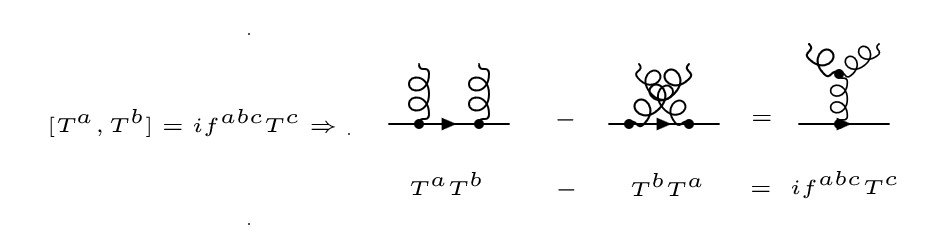
\includegraphics[scale=0.6]{images/Intro/Casimir.png}
\end{figure}
\item in the adjoint representation\\
\begin{figure}[h!]
\centering
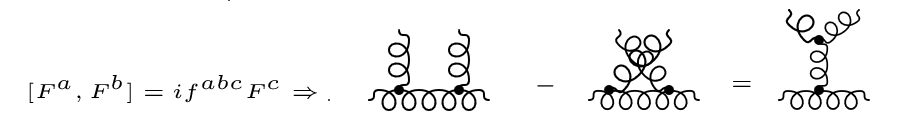
\includegraphics[scale=0.6]{images/Intro/CasimirAdj.png}
\end{figure}
\end{itemize}

The most common convention for the normalization of the generators in physics is:
\begin{equation}
\displaystyle\sum\limits_{c,d} f^{acd} f^{bcd} = N \delta^{ab}
\end{equation}
One of the most important equations for the colour factor calculation is the Jaccobi-Identity:
\begin{equation}
\begin{split}\:
[T^a, [T^b , T^c]]+[T^c, [T^a , T^b]]+[T^b, [T^c , T^a]]=0
\end{split}
\end{equation}
In terms of the structure constant:
\begin{equation}
\begin{split}\:
f^{axd} f^{bcx} +  f^{cxd} f^{abx} +f^{bxd} f^{cax} =0
\end{split}
\end{equation}

\begin{equation}
f^{abc} = -2i\: tr(T^a[T^b, T^c])
\end{equation}
%Which generalises to:
%\begin{equation}
%f^{abc}f^{xcd} = 4i\: tr(T^a[T^b, [T^c, T^d]])
%\end{equation}
\newpage
With these relations all Casimir operators can be calculated:

\begin{itemize}
\item Fundamental representation Casimir operator\\
\begin{figure}[h!]
\centering
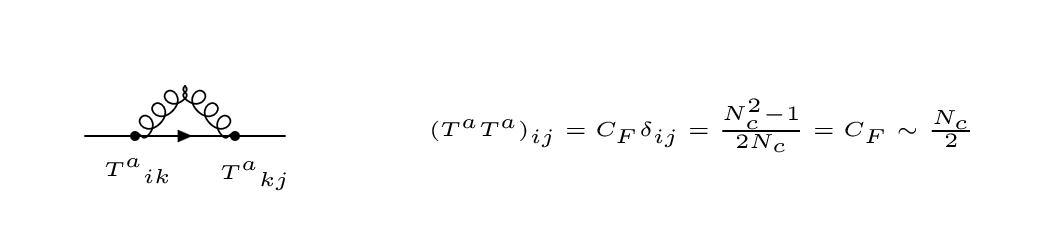
\includegraphics[scale=0.6]{images/Intro/Casimir1.png}
\end{figure}

\item Adjoint representation Casimir operator\\
\begin{figure}[h!]
\centering
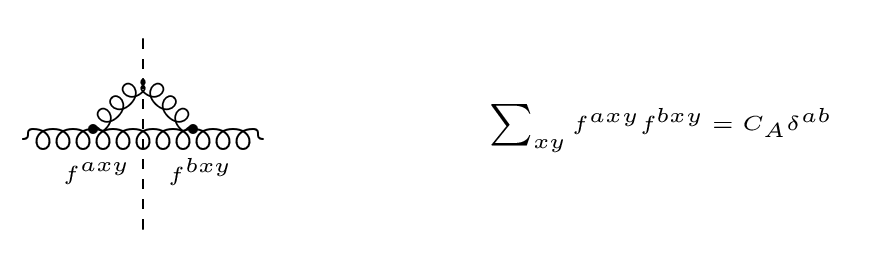
\includegraphics[scale=0.6]{images/Intro/Casimir2.png}
\end{figure}


Which means the charge of the gluon is twice that of the quark because:
\begin{equation}
 C_A = N_c =2C_F \sim 2(\frac{N_C}{2}) 
\end{equation}
\item Trace identities:\\
\begin{figure}[h!]
\centering
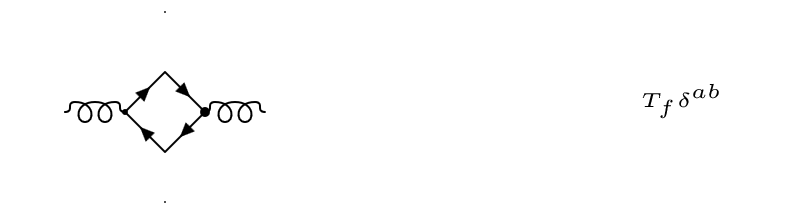
\includegraphics[scale=0.6]{images/Intro/Casimir3.png}
\end{figure}
\begin{figure}[h!]
\centering
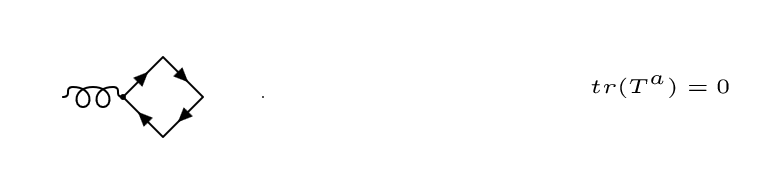
\includegraphics[scale=0.6]{images/Intro/Casimir4.png}
\end{figure}

\item Fierz identity
\end{itemize}
\begin{equation}
\displaystyle\sum\limits_{a} {T_{ij}}^a {T_{kl}}^a = \frac{1}{2}(\delta_{il}\delta_{kj}-\frac{1}{N}\delta_{ij}\delta_{kl})
\label{Fierz}
\end{equation}
With this identity the difference between QED and QCD can be clarified. The charge transfer in QED takes place along the Fermion line because photons cannot transport charges. On the other hand, the gluons transfer color charges. 
\begin{figure}[h!]
\centering
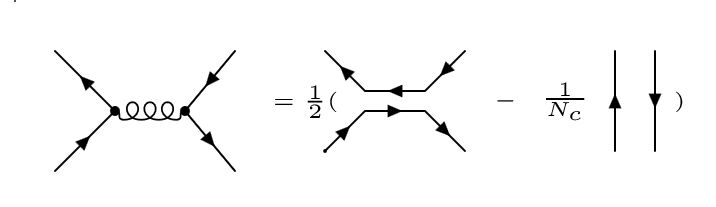
\includegraphics[scale=0.6]{images/Intro/Fritz.png}
\end{figure}
 

Other useful relations for the calculation of casimir operators in SU(N):
\begin{equation}
tr(T^a T^b)= {T_{ij}}^a {T_{ji}}^b = T_F \delta^{ab}
\end{equation}
\begin{equation}
\displaystyle\sum\limits_{a} (T^a T^a) = C_F \delta^{ij}
\end{equation}
\begin{equation}
f^{acd} f^{bcd} = C_A \delta^{ab}
\end{equation}
With $  T_F = \frac{1}{2} $ , $ C_A = N $ and $ C_F = \frac{N^2 -1}{2N} $
\pagebreak
\section{IR and Collinear Divergences}
\label{ir}
Beyond the LO (Leading order) diagrams based on massless particles, singularities occur. Consider first the process $ e^- e^+ \rightarrow q\bar{q}g $

\begin{figure}[ht!]
\centering
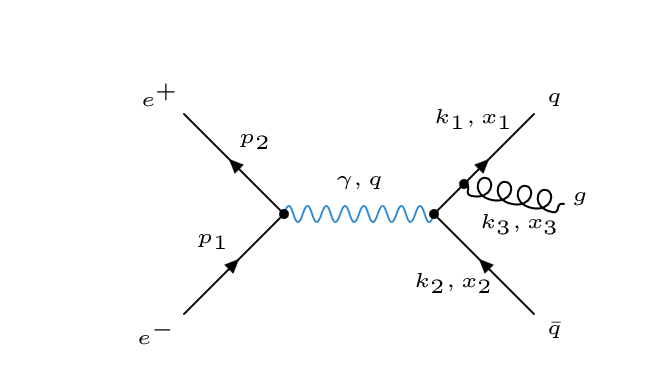
\includegraphics[width=0.6\textwidth]{images/Intro/IRCol.png}
\end{figure}

In order to calculate the cross section of electron-positron annihilation, regard the gluon emission from a parent (anti)quark. The amplitude of this process fig. \ref{IRCo} is:
\begin{figure}[h!]
\centering
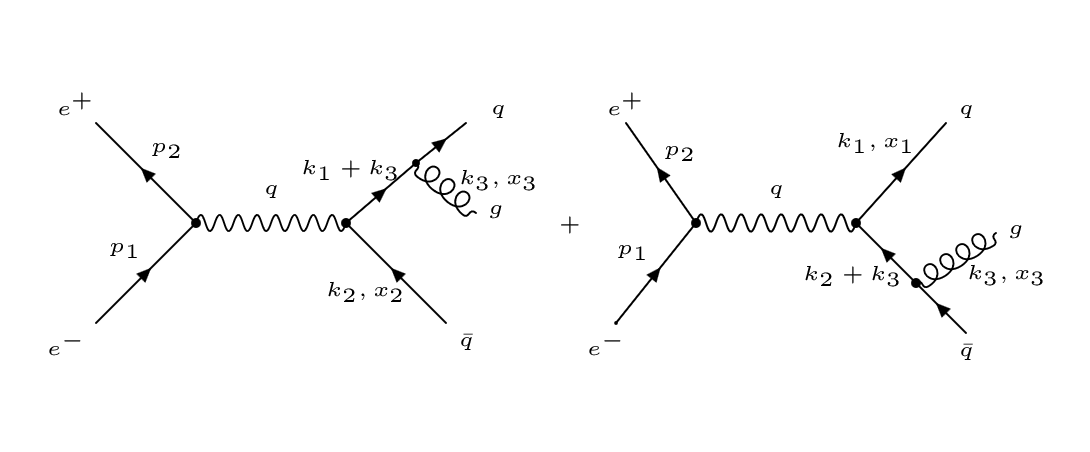
\includegraphics[width=0.85\textwidth]{images/Intro/IRColMatrix.png}
\caption{Left diagram $  e^- e^+ \rightarrow qg\bar{q} $ and right $ e^- e^+ \rightarrow q\bar{q}g $}
\label{IRCo}
\end{figure}

\begin{equation}
\begin{split}
A = & \frac{\bar{u}(k_1)(-ig_s\gamma^{\nu}\times T^a)[-i(\not{k_1}+\not{k_3})](-iee_q \gamma^{\mu})v(k_2){\epsilon_{\mu}}^{\lambda_1}{\epsilon_{\nu}}^{\lambda_2*}}{(k_1 + k_3)^2}\\ 
&- \frac{\bar{u}(k_1)(-iee_q \gamma^{\mu})[i(\not{k_2}+\not{k_3})](-ig_s\gamma^{\nu}\times T^a)v(k_2){\epsilon_{\mu}}^{\lambda_1}{\epsilon_{\nu}}^{\lambda_2*}}{(k_1 + k_3)^2}\\
\Rightarrow &A=-g_s T^a[ \frac{\bar{u}\:\not{\epsilon}\:(\not{k_1}+\not{k_3})\:\Gamma \:v}{(k_1 + k_3)^2} - \frac{\bar{u}\:\Gamma\:(\not{k_2}+\not{k_3})\:\not{\epsilon} \:v}{(k_2 + k_3)^2}]
\end{split}
\end{equation}
With $\Gamma=(-iee_q \gamma^{\mu}){\epsilon_{\mu}}^{\lambda_1}$.\\
Considering massless partons, the amplitude can be written:
\begin{equation}
 A=-g_s T^a[ \frac{\bar{u}\:\not{\epsilon}\:(\not{k_1}+\not{k_3})\:\Gamma \:v}{2k_1 \cdot k_3} - \frac{\bar{u}\:\Gamma\:(\not{k_2}+\not{k_3})\:\not{\epsilon} \:v}{2k_2 \cdot k_3}]
\end{equation}
In the soft limit with $k_0 \rightarrow 0$, the amplitude can be factorized in two parts:
\begin{equation}
 A=-g_s T^a[ \frac{k_1\:{\epsilon}}{k_1 \cdot k_3} - \frac{k_2\:{\epsilon}}{k_2 \cdot k_3}] A_{born} \:\:\:\:\:\:\:\:\:\:\:\:\:\:\:\:\:\text{with}\:\: A_{born}= \bar{u}\: \Gamma \:v
\end{equation}
Where the left side contains all information about colour and momenta and the other one involves all spin information.
The calculation of the cross section results in:
\begin{equation}
\begin{split}
\sigma=&-C_F g_s^2 \sigma^{born} \int \frac{d^3 k}{2k_0 (2{\pi})^3} 2(\frac{k_1 \cdot k_2}{(k_1 \cdot k_3)(k_2 \cdot k_3)})\\ 
&-C_F g_s^2 \sigma^{born} \int dcos\: \theta\: \frac{d k_0}{k_0} \frac{4}{(1-cos\: \theta)(1+cos\: \theta)}
\label{cr}
\end{split}
\end{equation}
In the Center of Mass frame the total energy is defined by $ \sqrt{s} $. With $ q^{\mu} $ the virtual photon momentum  is achieved $ q^2 =2 $. In order to simplify the above equation \ref{cr} it is useful to define energy fractions $ x_i $ as:
\begin{equation}
x_i = \frac{2E_i}{\sqrt{s}}=\frac{2q\: \cdot\: k_i}{s}
\end{equation}
With the energy conservation can be obtained $ \sum x_i =2  $ and Consequently, it is noted that only two moments are independent. So, the angle $ \theta_{ij} $ between the momenta of partons $ i $ and $ j $ can be related to the momentum fractions as follows \cite{Soper:1996fy}

\begin{equation}
\begin{split}
2k_i \cdot k_j =& (k_i+k_j)^2 = (q-k_k)^2 = s-2q \cdot k_k\\
&2E_i E_j (1-cos \theta_{ij})=s(1-x_k)
\end{split}
\end{equation}
Dividing these equations by $ s/2 $, one receives:
\begin{equation}
x_i x_j (1-cos \theta_{ij})=2(1-x_k)
\end{equation}
This allows the partonic differential cross section to be rewritten as:
\begin{equation}
\frac{d^2 \sigma}{dx_1 dx_2}= (\frac{4\pi \alpha}{s})\sum {e_i}^2 
\frac{2\alpha_s}{3\pi} \frac{{x_1}^2+{x_2}^2}{(1-x_1)(1-x_2)}
\label{fully}
\end{equation}

As can be seen, there are three singularities within the final result. 
If the emitted photon is collinear to the outgoing quark or anti-quark $ (x_1 \rightarrow 1 \:\text{or}\: x_2 \rightarrow 1) $ and when the emitted gluon is soft $ (x_1 \rightarrow 1\: \text{and}\: x_2 \rightarrow 1 )$.
\newpage
The singularities come from the quark propagator in each diagram. The denominators contain terms proportional to $ \frac{1}{(k_i + k_j)^2}  $. Without the neglectable quark mass follows:
\begin{equation}
\frac{1}{(k_i + k_j)^2}=\frac{1}{2k_i \cdot k_j}=\frac{1}{2E_iE_j(1-cos\theta_{ij})}=\frac{1}{s(1- x_k)}
\end{equation} 


With $ x_3= 2-x_1-x_2 $ and the relations $ 0\leq x_i < 1 $ it can be implied that the allowed region for the phase space is a triangle. All possibilities for three partons in the phase space is shown in figure \ref{conf}:

\begin{figure}[h!]
\centering
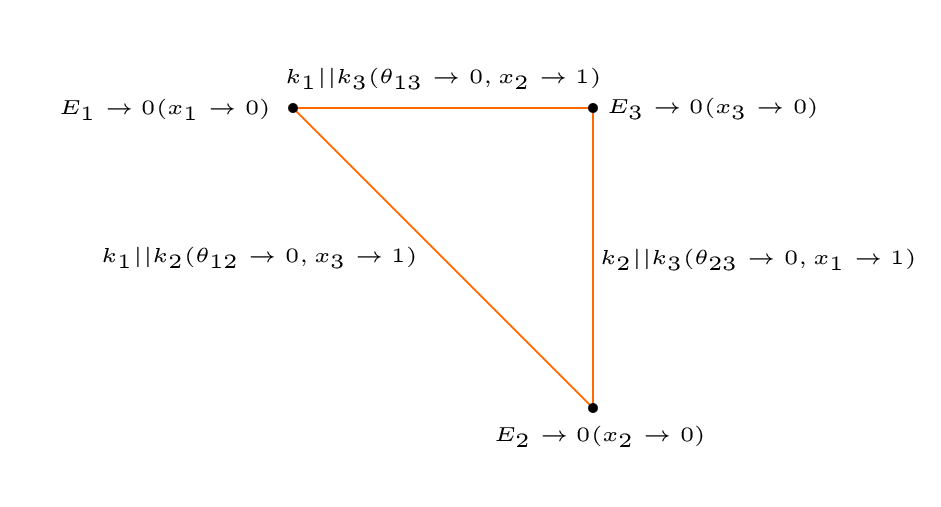
\includegraphics[scale=0.6]{images/Intro/triangle.png}
\caption{Three-parton configurations in the phase space.
The edges $ x_i= 1 $ show the collinear regions for two partons. The corners $ x_i= 0 $ correspond to one parton momentum being soft}
\label{conf}
\end{figure}

The Kinoshita-Lee-Nauenberg (KLN) \cite{Grandou:1994rz} Theorem assures that a summation over degenerate initial and final states removes all infrared (IR) divergences and the sum of the integrals $ \int_R $ and $ \int_V $ over the phase space is finite. However, this is not true for the individual contributions.
\begin{figure}[h!]
\centering
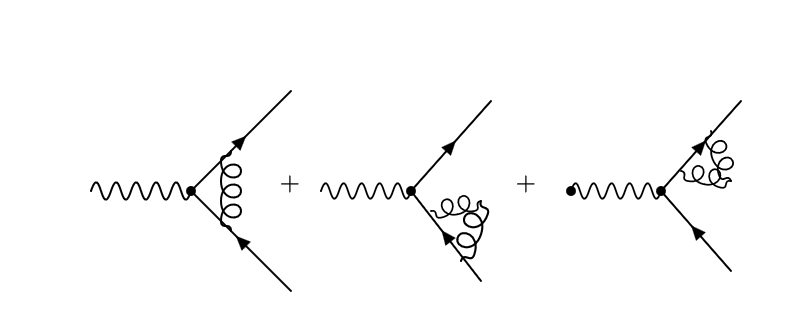
\includegraphics[scale=0.5]{images/Intro/virtual.png}
\caption{Virtual corrections: one-loop corrections to $  e^- e^+ \rightarrow q\bar{q} $}
\end{figure}



\section{Hard scattering}
\label{Hard scattering}
In the last section it was seen that IR singularities occur in QCD due to the collinearity of two partons or the soft energy of a parton. These divergences happen long time after the initial hard scattering (long distance physics). Since the infrared-safe observables are calculable in perturbative QCD, the factorisation theorem can be applied to remove the singularities from the partonic cross section of the long-distance physics and absorbed into the parton distribution of the hadrons. This is even feasible for all orders of calculation. Consider the hadron hadron scattering:
\begin{equation}
\sigma = \sum_{ij} \int dx_1 dx_2 f_i(x_1, \mu^2)f_j(x_2, \mu^2) \sigma_{ij}(x_1, x_2, Q^2/\mu^2... )
\end{equation}
\begin{figure}[h!]
\centering
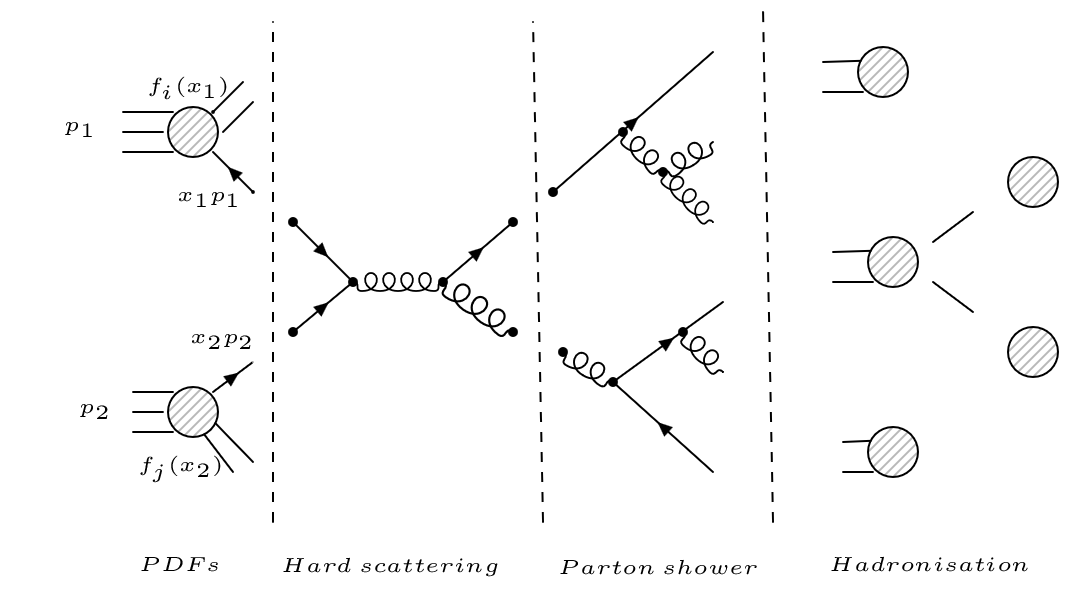
\includegraphics[width=0.85\textwidth]{images/Intro/Hard.png}
\end{figure}
With a factorisation scale $ \mu $ the long and short-distance physics could be separated. Partons with a greater momentum than $ \mu $ participate in the hard-scattering and those with less momentum are considered as components of the hadron structure and accordingly absorbed in the parton distribution ~\cite{Nagy:2006kb}.\\
The factorisation theorem also applies to deep inelastic scattering,
with one of the parton distributions replaced by an $ e^+ e^- \gamma $ vertex. The DIS cross section can be written as ~\cite{Ellis:1991qj}
\begin{equation}
\frac{d^2 \sigma}{dx dQ^2}=\frac{4\pi \alpha^2}{x Q^4}[(1-y)F_2 (x, Q^2)+xy^2 F_1(x, Q^2)]
\end{equation}
In this case, the structure function needs to be introduced: 

\begin{equation}
{{F}_2}^{exp} (x)= \sum_i {e_i}^2 x f_i(x)
\end{equation}
\pagebreak
It is defined as the charge weighted sum of the parton momentum densities which describe the probability that the parton carries a momentum
fraction between $ x $ and $ d x $ of the proton momentum. The index $i$ denotes the quark flavour. Parton distributions are non-pertubative. Fortunately, they are universal and obtainable from a fit to the data for a particular factorisation scheme and usable in other processes.\\
The perturbative evolution kernel of a parton distribution due to splitting can be described by the solution of DGLAP evolution equation~\cite{Ward:1995xy}. It is based on the collinear factorisation property of QCD. Fixing the accuracy of the calculation and the factorisation scheme the evolution kernel is well defined.  
\begin{equation}
\frac{\partial f(x, \mu^2) }{\partial \: ln \:\mu^2}=
\frac{\alpha_s}{2\pi}\int_{x}^{1}\frac{dy}{y} f_j(y, \mu^2) P_{ij}(\frac{x}{y})+O({\alpha_s}^2)
\end{equation}
This is a system of coupled integral or differential equations. $ P_{ij}(\frac{x}{y}) $ represents the probability, a daughter parton $ i $ with momentum fraction $ \frac{x}{y} $ is splits from a parent parton $ j $.
The above convolution in compact notation (Mellin Convolution) in the general case:
\begin{equation}
\frac{\partial f_i(x, \mu^2) }{\partial \: ln \:\mu^2}=
\sum_{j=-n_f}^{n_f} P_{ij} \otimes f_j(\mu^2)
\end{equation}

The four splittings probabilities are illustrated in the diagram \ref{splitting} and the qq, qg, gg and gq transitions lead to a set of $ 2n_f +1 $ coupled evolution equations.
\begin{equation}
\frac{\partial }{\partial \: ln \:\mu^2} \left(\begin{array}{c}q_s\\ g\end{array}\right)=
\frac{\alpha_s}{2\pi}\begin{bmatrix}P_{qq} & 2n_fP_{qg} \\P_{gq} & P_{gg} \end{bmatrix}\otimes\left(\begin{array}{c}q_s\\ g\end{array}\right)
\end{equation}

A parton distribution changes when a different parton splits or the parton itself splits. Parton densities can not be analytically determined, but it is possible to predict how they evolve from one scale to another. PDFs are measured in one process and can be used as an input for another process.


\begin{figure}[h!]
\centering
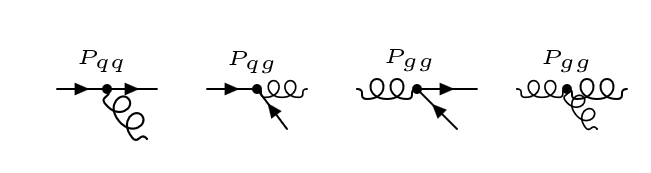
\includegraphics[width=0.85\textwidth]{images/Intro/spiliting.png}
\caption{The four splitting probabilities}
\label{splitting}
\end{figure}
The  spin-averaged  unregularized  Altarelli-Parisi  splitting  functions  in $ d $-dimensions  are given by:
\begin{equation}
	\left.\begin{aligned}
\langle\:\hat{P_{qq}}\rangle &= C_F[\frac{1+z^2}{1-z}-\varepsilon(1-z)]\\
\langle\:\hat{P_{gq}}\rangle &= T_R[1-\frac{2z(1-z)}{1-\varepsilon}]\\
\langle\:\hat{P_{qg}}\rangle &= C_F[\frac{1+(1-z)^2}{z}-\varepsilon z]\\
\langle\:\hat{P_{gg}}\rangle &= 2C_A[\frac{z}{1-z}+\frac{1-z}{z}+z(1-z)]
\end{aligned}
	\right\}
	\quad \text{Alterali-Parisi
	}
\label{Alterali-Parisi}
\end{equation}


\section{Subtraction method}
The subtraction term is constructed as a sum over all possible dipole configurations, i.e. all possible combinations of two partons are formed to build an emitter while every single one of the remaining partons is considered a spectator. The general quadratic matrix element is defined as:
\begin{equation}
|A|^2 = |{A^{(0)}}_m|^2 +  |{A^{(0)}}_{m+1}|^2+ 2Re({A^{(0)*}}_{m}{A^{(1)}}_{m})
\end{equation}
Where $ |{A^{(0)}}_m|^2 $ is the tree level contribution (Born sector) from LO and has no divergences, $ |{A^{(0)}}_{m+1}|^2+ 2Re({A^{(0)*}}_{m}{A^{(1)}}_{m}) $ comes from NLO and each of them is divergent. The problem in this case is the Integrals which can not be combined due to different phase space dimensions:

\begin{equation}
\sigma^{NLO} = \int_{m+1} d \sigma^R +\int_{m} d \sigma^V
\end{equation}
The real and virtual contributions are both IR divergent and need to be regularised in $ d = 4-2\epsilon $ dim.
To tackle this problem one can use the subtraction method with adding and subtracting a local counter term $ d \sigma^A $ with the same singularity structure as term $ d \sigma^R $ to the integral. $ d \sigma^A $ approximates the soft and collinear singularities of $ d \sigma^R  $.
\begin{equation}
\sigma^{NLO} = \int_{m+1} [d \sigma^R -d \sigma^A]+\int_{m} [d \sigma^V+\int_1 d \sigma^A]
\end{equation}
In this case, one can safely set $ \epsilon \rightarrow 0 $ for $ d \sigma^R |_{\epsilon \rightarrow 0}  -d \sigma^A |_{\epsilon \rightarrow 0} $ under the integral sign in the first term and calculate the integral numerically in 4-dimensions. All the singularities are now associated to the last two terms on the right-hand side. If one is able to carry out analytically the integration of $ d \sigma^A $ over one parton subspace leading to the $ \epsilon $ poles, one can combine these poles with those in $ d \sigma^V $, thus cancelling all the divergences, performing the limit $ {\epsilon \rightarrow 0} $ and carrying out numerically the remaining integration over the $ m $-parton phase space \cite{Catani:2002hc}. 
\begin{equation}
\sigma^{NLO} = \int_{m+1} [d \sigma^R |_{\epsilon \rightarrow 0}  -d \sigma^A |_{\epsilon \rightarrow 0}]+\int_{m} [d \sigma^V+\int_1 d \sigma^A]_{\epsilon \rightarrow 0}
\end{equation}
The virtual contribution must be UV-finite:
\begin{equation}
\int_{m} d \sigma^V= \int_m [\int d {\sigma^V}_{bare} + {\sigma^V}_{Counter\:term}]
\end{equation}
The addition of $\int_1 d \sigma^A$ to the $ \int_{m} d \sigma^V $ ensures that IR poles are cancelled.
The bare and counter contribution are separately divergent and have also different integral dimensions. One can use the same idea with the subtraction method to solve this problem~\cite{Catani:1996vz}
\begin{equation}
\int_{m} d \sigma^V +\int d {\sigma^L}-\int d {\sigma^L}= \int_m \int[ d {\sigma^V}_{bare}- \partial {\sigma^L}] + \int_m[{\sigma^V}_{Counter\:term}+ \int d {\sigma^L}]
\end{equation}

together one receives:

\begin{equation}
\sigma^{NLO} = \int_{m+1} [d \sigma^R -d \sigma^A]+ \int_m \int [ d {\sigma^V}_{bare}- d {\sigma^L}] + \int_m[{\sigma^V}_{Counter\:term}+ \int d {\sigma^L}+d \sigma^A]
\end{equation}

\section*{Determination of emission kernels}
The counter term $ d \sigma_A $ must approximate soft and collinear singularities of $ d \sigma_R $ in d dimensions. This process and specific observable has to be obtained in a way that is independent of the particular jet observable considered. It must be exactly integrable analytically over one-parton phase space in d and $ d \sigma_R -  d \sigma_A  $ has to be integrable via Monte Carlo methods. $ d \sigma_A $ acts as a local counter-term for $ d \sigma_B $ at this point. One derives improved factorisation formulae which are called dipole or antenna formulae:
\begin{equation}
d \sigma_A = \sum_{dipoles} d \sigma_{B} \times d V_{dipoles}
\end{equation}
Where the sum is over dipoles for all $ m+1 $ configurations with consideration to a given m-parton state. $  d \sigma_{B}$ describes the color/spin projection of the Born-level exclusive cross section.
The symbol $ \times $ describes phase space convolutions and sums over colour and spin indices. $ d V_{dipoles} $ will be computed and its singular properties matched to the real part. The Dipoles are universal in the sense that they do not depend on the hard scattering. This allows the use of a factorisable mapping from
the $m + 1$-parton phase space to an $m$-parton subspace. That will be clearer when the parametrisation is used in the next chapter. 
The integral over all $ m+1 $ configuration can be written:
\begin{equation}
\int_{m+1}d \sigma_A =  \int_{m} d \sigma_{B} \times \sum_{dipoles} \int_{1}d V_{dipoles}
\end{equation}
This is the important result because this can now be written in terms of the known $ m $-sector from LO and the other universal factor which contains all $ \epsilon $-poles \cite{Catani:2002hc}.
\section*{Singularity Structure}

Before beginning with the collinear limit or soft limit respectively the structure of the matrix element from LO has to be introduced:

\begin{equation}
{\mathcal{M}_m}^{c_1,...,c_m;s_1,...,s_m}(p_1,..., p_m)
\end{equation}

$ c_i $, $ s_i $ and $ p_i $ denote respectively the colour, spin indices and the momenta for each\\ $m$-parton in the tree level matrix element in the initial/final-state. A common used method here is to define a basis in colour+helicity space.
\begin{equation}
{\mathcal{M}_m}^{c_1,...,c_m;s_1,...,s_m}(p_1,..., p_m)\equiv(<c_i,..,c_m|\otimes <s_1,...,s_m|)|1,..,m>_m
\end{equation}
With $ <c_i,..,c_m|\otimes <s_1,...,s_m|)| $ as the basis and $ |1,..,m>_m $ as a vector in this space.
Thus, for the matrix element squared:

\begin{equation}
\begin{split}
\vert \mathcal{M}_m \vert^2=& (< c_i,..,c_m | \otimes < s_1,...,s_m|)(| c_i,..,c_m > \otimes | s_1,...,s_m >) < 1,..,m | 1,..,m > \\
&=\delta_{c_1 c_1},...\delta_{c_m c_m} \otimes \delta_{s_1 s_1},...\delta_{s_ms_m} \:_m < 1,..,m | 1,..,m > \:_m
\end{split}
\end{equation}
Define a colour-charge operator  $ {T_i} $ with the
emission of a gluon from each parton i:
\begin{equation}
\begin{split}
T_i = {T_i}^c |c>
\end{split}
\end{equation}
Its action onto the colour space is defined by:

\begin{equation}
<c_1,..,c_i,..c_m,c|T_i|b_1,..,b_i,..b_m>=\delta_{c_1b_1}...{T^c}_{c_ib_i}
...\delta_{c_mb_m}
\end{equation}

Where $ {T^c}_{c_ib_i} $ is the colour-charge matrix in the adjoint representation for the gluon emission or colour-charge matrix in the fundamental representation for the quark/anti-quark emission case. The following properties must be taken into account:
\begin{equation}
\begin{split}
&T_i \cdot T_j = T_j \cdot T_i \:\:\:\:\:\:\:\:\:\:\:\:\:\:\:\:\:\:\:\:\text{if}\:i\neq j,\: \text{commutative property}\\
& {T_i}^2 = C_i\:\:\:\:\:C_i = C_A \:\:\:\:\:\:\:\:\:\:\:\text{for gluon and} \: C_i = C_F\:\text{for (anti)quark}\\
&\sum_{i=1}^m T_i |1,...,m>_m =0 \:\:\:\:\:\text{for single state}
\end{split}
\end{equation}
Thus, the square of colour-correlated tree-amplitudes for the indices $I,  J$ referring either to final-state or initial-state partons will be~\cite{Catani:1996vz, Catani:2002hc}
\begin{equation}
\vert {{\mathcal{M}}^{I,J}}_{m,a...} \vert^2=\:_{m,a...} < 1,...,m;a,... |T_I \cdot T_J | 1,...,m;a,... >\:_{m,a...}
\end{equation}


\pagebreak
\section*{Dipole factorisation}
Depending on the investigated region, there is a total of three factorisation possibilities, see figures \ref{soft}, \ref{Collinear} and \ref{Dipole}.
\begin{figure}[h!]
\centering
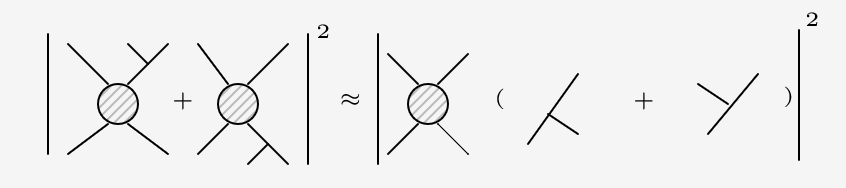
\includegraphics[width=0.85\textwidth]{images/Intro/soft.png}
\caption{Soft factorisation}
\label{soft}
\end{figure}

\begin{figure}[h!]
\centering
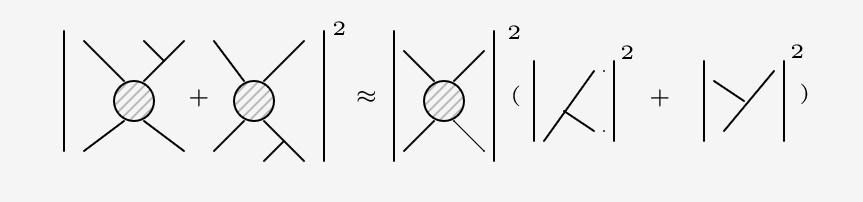
\includegraphics[width=0.85\textwidth]{images/Intro/collinear.png}
\caption{Collinear factorisation}
\label{Collinear}
\end{figure}

\begin{figure}[h!]
\centering
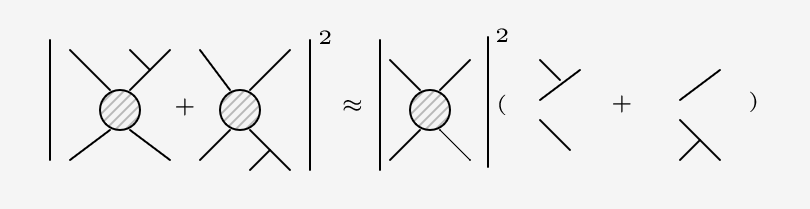
\includegraphics[width=0.85\textwidth]{images/Intro/factorization.png}
\caption{Dipole/Antenna factorisation}
\label{Dipole}
\end{figure}
To explain the meaning of the factorisation consider $(m+1)$-partons with the general matrix element~\cite{Seymour:1994we, Catani:2002hc}
\begin{equation}
\vert {{\mathcal{M}}}_{m+1} (Q; p_1,...,p_i,...,p_j,...,p_{m+1}) \vert^2
\end{equation}

In the soft region the momentum $ p_j $ can be parametrised with $ p_j \rightarrow \lambda q, \lambda \rightarrow 0 $, where $ q $ is an arbitrary four vector and $ \lambda $ a scale parameter. 
The squared matrix element is characterised by $ \vert {{\mathcal{M}}} \vert^2 \sim \frac{1}{\lambda^2}$. If $ p_i $ and $ p_j $ become collinear, the parametrisation $ p_j = \frac{z}{1-z} p_i $ will be chosen. So the matrix element will be $ \vert {{\mathcal{M}}} \vert^2 \sim \frac{1}{p_i \cdot p_j}$.
This get covered in more detail in the next chapter. Here a summery of the behaviour of the matrix elements in different regions is given.
Based on the Catani-Seymour method for $(m+1)$-partons. 
\begin{equation}
\vert {{\mathcal{M}}}_{m+1}  \vert^2 \rightarrow \sum \vert {{\mathcal{M}}}_{m}  \vert^2 \times V_{ij,k}
\Rightarrow \vert {{\mathcal{M}}}_{m+1}  \vert^2 \rightarrow \sum \vert {{\mathcal{M}}}_{m}  \vert^2 \times V_{ij,k}
\end{equation}

$ V_{ij,k} $ a singular factor including parton $k$ and its interaction with partons $i$ and $j$ from the $m$-parton amplitude. This situation can be represented by the diagram \ref{factorisationPic}.

\begin{figure}[h!]
\centering
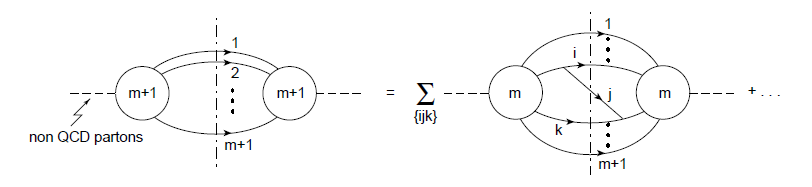
\includegraphics[width=0.85\textwidth]{images/Intro/factorisationPic.png}
\caption{Factorisation in dipole formalism}
\label{factorisationPic}
~\cite{Catani:1996vz}
\end{figure}

Here $i$ and $j$ are the emitters and k plays the role of a spectator. The spectator absorbs a longitudinal recoil that arises when a splitting is performed with  all  participating  partons  remaining  on  their  mass  shells. The blobs denote the tree-level matrix elements and their complex conjugate. The dots on the right-hand side stand for non-singular terms both in the soft and collinear limits.
When the partons i and j become soft and/or collinear, the singularities are factorized into the term $ V_{ij,k} $ (the
dashed box on the right-hand side) which embodies correlations with a single additional parton k.

\begin{figure}[h!]
\centering
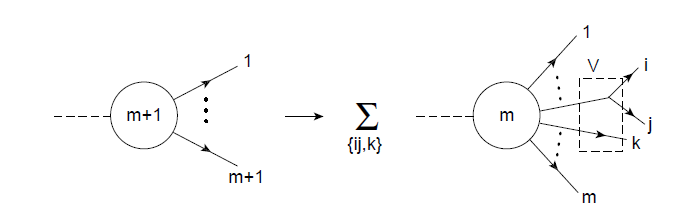
\includegraphics[width=0.85\textwidth]{images/Intro/factorisationPic2.png}
\caption{Effective diagrams for the different emitter–spectator cases.}
\label{factorisationPic2}
~\cite{Catani:2002hc}
\end{figure}

In this context the different dipole factorisation for both initial states and final states shall be presented. All these different possibilities can be seen in the diagram \ref{factorisationPic2}.
$  \mathcal{D}_{ij,k} $ describes the final state emitter and final-state spectator (FF), $  {\mathcal{D}^a}_{ij} $ the final-state emitter and initial-state spectator (FI), $ {\mathcal{D}^{ai}}_{k} $ the initial-state emitter and final-state spectator (IF) and $ \mathcal{D}^{aj,b} $ the initial-state emitter and initial-state spectator (II).
The dipole factorisation formula for all these possibilities is \cite{Schumann:2007mg}
 \begin{equation}
 |\mathcal{M}_m+1|^2 = \displaystyle\sum\limits_{i,j} \displaystyle\sum\limits_{k\neq i,j} \mathcal{D}_{ij,k} +\displaystyle\sum\limits_{i,j} \displaystyle\sum\limits_{a} {\mathcal{D}^a}_{ij}+\displaystyle\sum\limits_{a,i} \displaystyle\sum\limits_{k\neq i} {\mathcal{D}^{ai}}_{k}+\displaystyle\sum\limits_{a,i} \displaystyle\sum\limits_{b\neq a} \mathcal{D}^{aj,b}+...
 \end{equation}
In each term $ i, j $ and $ k $ denote final-state partons and a and b stand for initial-state partons. Note that there are many non-divergent contributions or diagrams, which are marked here with the dots. In this work the first contribution final-state emitter and final-state spectator (FF) is used. Later it becomes clear how to deal with the formula.

\begin{figure}[h!]
\centering
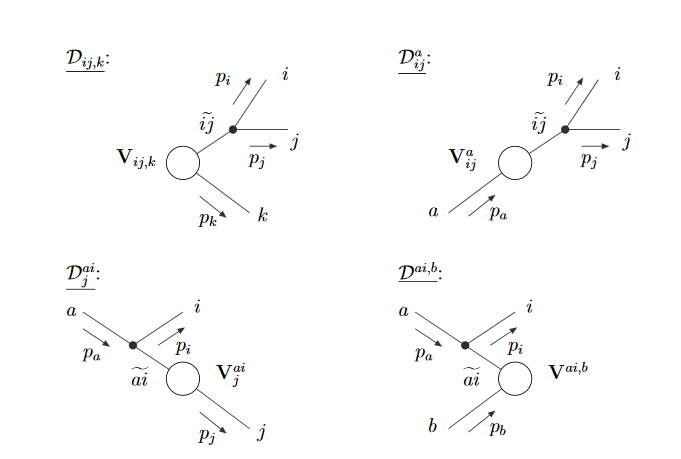
\includegraphics[width=0.85\textwidth]{images/Intro/Dipole.png}
\end{figure}

The circle in the center of each sub diagram presents the $m$-partons matrix element and the tilde labels the collinear splitting process for the initial or final states.
For this work, the first upper diagram with final-state singularities without initial-state partons, is completely sufficient and is discussed here in detail with its formula.
The matrix element for this is written:

\begin{equation}
\vert {{\mathcal{M}}}_{m+1}  \vert^2 = < 1,...,m+1 || 1,...,m+1 > = \sum_{k \neq i,j} {{\mathcal{D}}}_{ij,k}(p_1,...,p_{m+1}) +\text{finite terms}
\end{equation}

The first term with the sum over dipoles is divergent as $ p_i \cdot p_j \rightarrow 0 $. 
For the case of final-state emitters with a final-state spectator, for instance, the individual dipole contributions:
\begin{equation}
 {{\mathcal{D}}}_{ij,k}(p_1,...,p_{m+1}) = \frac{-1}{2p_i \cdot p_j} \:\:_m<1,...,\tilde{ij},...,k,...,m+1 |\frac{T_k \cdot T_{ij}}{{T_{ij}}^2} V_{ij,k}| 1,...,\tilde{ij},...,k,...,m+1 >\:_m
\end{equation}

Where $ T_k \cdot T_{ij} $ are the color charges of spectator and emitter, $ V_{ij,k} $ splitting kernel in helicity space of emitter
explicit form depends on parton type become proportional to Altarelli-Parisi splitting functions \ref{Alterali-Parisi} and eikonal factors
in collinear and soft limits.\\
The occurring $ m $-parton states are constructed from the original $(m+ 1)$-particle matrix element by replacing the partons $ i $ and $ j $ with the new parton $  \widetilde{ij} $ , and the original parton $ k $ with the $  \widetilde{k} $ spectator. In the massless case, their momenta are given by:

\begin{equation}
\begin{split}
&{\tilde{p}^{\mu}}_{ij} = {p_i}^{\mu}+{p_j}^{\mu}-\frac{y_{ij,k}}{1-y_{ij,k}}{p_k}^{\mu}\\
&{\tilde{p}^{\mu}}_{k} = \frac{1}{1-y_{ij,k}}{p_k}^{\mu}\\
&y_{ij,k}=\frac{p_i \cdot p_j}{p_i \cdot p_j+p_j \cdot p_k+p_k \cdot p_i}
\end{split}
\end{equation}

Note, that momenta are on-shell. Due to momentum conservation\\ ${p_i}^{\mu}+{p_j}^{\mu}+{p_k}^{\mu}= {\tilde{p}^{\mu}}_{k} +{\tilde{p}^{\mu}}_{ij} $. 
